\section{电子对重建}

当可能是电子或者正电子的径迹被挑选出来之后,就需要对正负电子进行配对来得到电子对的不变质量(Invariant mass,\Mee)和横动量(\pt)分布。由于在末态并不能知道哪些正负电子是来于自同一个过程(例:来自于同一个介子衰变而来的电子和正电子),只能对同一个事例中所有的正负电子进行随机配对得到异号分布(UnLike-Sign distribution, ULS, \Npm)。这样就会引入大量的背景(Background)。在配对过程当中,背景主要有以下几种来源
\begin{itemize}
  \item 电子随机组合背景:由于随机配对,将来自于完全不同的两个过程的正负电子组合在一起。例如将一个来自于$\omega$两体衰变的电子和一个来自于$\phi$的电子进行配对。
  \item 关联背景:将有一定关联性但并不是同一个衰变过程中的正负电子进行配对。其并不能完全地反应母粒子的信息。例如当$\pi^0$发生Dalitz衰变时产生的光子继续衰变成两个电子时($\pi^0\rightarrow e^+ + e^- + \gamma \rightarrow e^+ + e^- + e^+ + e^- $),将末态由光子衰变产生的电子和Dalitz衰变时产生的电子配对,虽然其有一定的关联但并不是我们想要的信号。关联背景另外的一个来源是来自于同一个或者背对背喷注(Jet)的电子对。
  \item 光子转换背景:当光子打到探测器材料上的时候因为电子对效应所产生的电子对
\end{itemize}

基于同样的原因,背景也只能通过某种手段来估计其在异号分布当中所占的比例。在双轻子分析中,常用的背景估计方法主要有两种:同事例同号配对(Same event Like-Sign, LS, \Npp~or \Nmm)和混合事例配对(Mixed event)。在本分析中是使用同事例同号配对的方式来重建背景。因为TPC不同扇区(Sector)之间的支撑结构带来的接收度缺失,以及正负电子在相同的磁场下的偏转方向不同,这使得异号双电子对(unlike-sign pair)和同号双电子对(like-sign pair)之间的接收度存在差别。此时混合事例配对的方法被用来构建一个修正因子来修正这个接收度的差别。这几种不同的背景和重建方法将会在接下来的几个小节当中进行详细的讨论。

\subsection{同号配对方法}
同号配对方法和之前提到的异号电子对的配对方式类似,不同的是同好配对方法是将同一个事例当中电荷相同的电子进行随机配对,从而得到\Npp 和\Nmm 的分布。这种方法可以很好的重建关联背景和随机组合背景。但缺点是统计较少,和 \Npm 为一个数量级。在相同的磁场下,正电子和负电子的径迹向着相反的方向弯折,并且因为TPC的支撑结构的存在,在扇区和扇区之间有接收度的死区。这导致在电子和正电子有着相同的横动量的时候,两者的接收度并不相同,如图\ref{fig:Phi_vs_Q}所示。这样\Nmm 和 \Npp 与 \Npm 的接收度会有差别。这就需要进行电子对的接收度进行修正。电子对接收度修正因子($f_{pair~sign~acc.}$)通过混合事例方法(mixed event)得到,具体方法会在下一小节中介绍。\Npp 和 \Nmm 的几何平均数经过电子对接收度修正后,将用来估计背景并且在同号分布当中进行背景扣除。背景 $N_{bkg}$ 的计算方法如下式所示:
\begin{equation}
    N_{bkg} = \frac{B_{+-}}{2\sqrt{B_{++}B_{--}}}*2\sqrt{N_{++}N_{--}}
\end{equation}

其中$\frac{B_{+-}}{2\sqrt{B_{++}B_{--}}}$ 为电子对接收度修正因子,将在下一小节中介绍。

\begin{figure}[htb]
  \begin{center}
  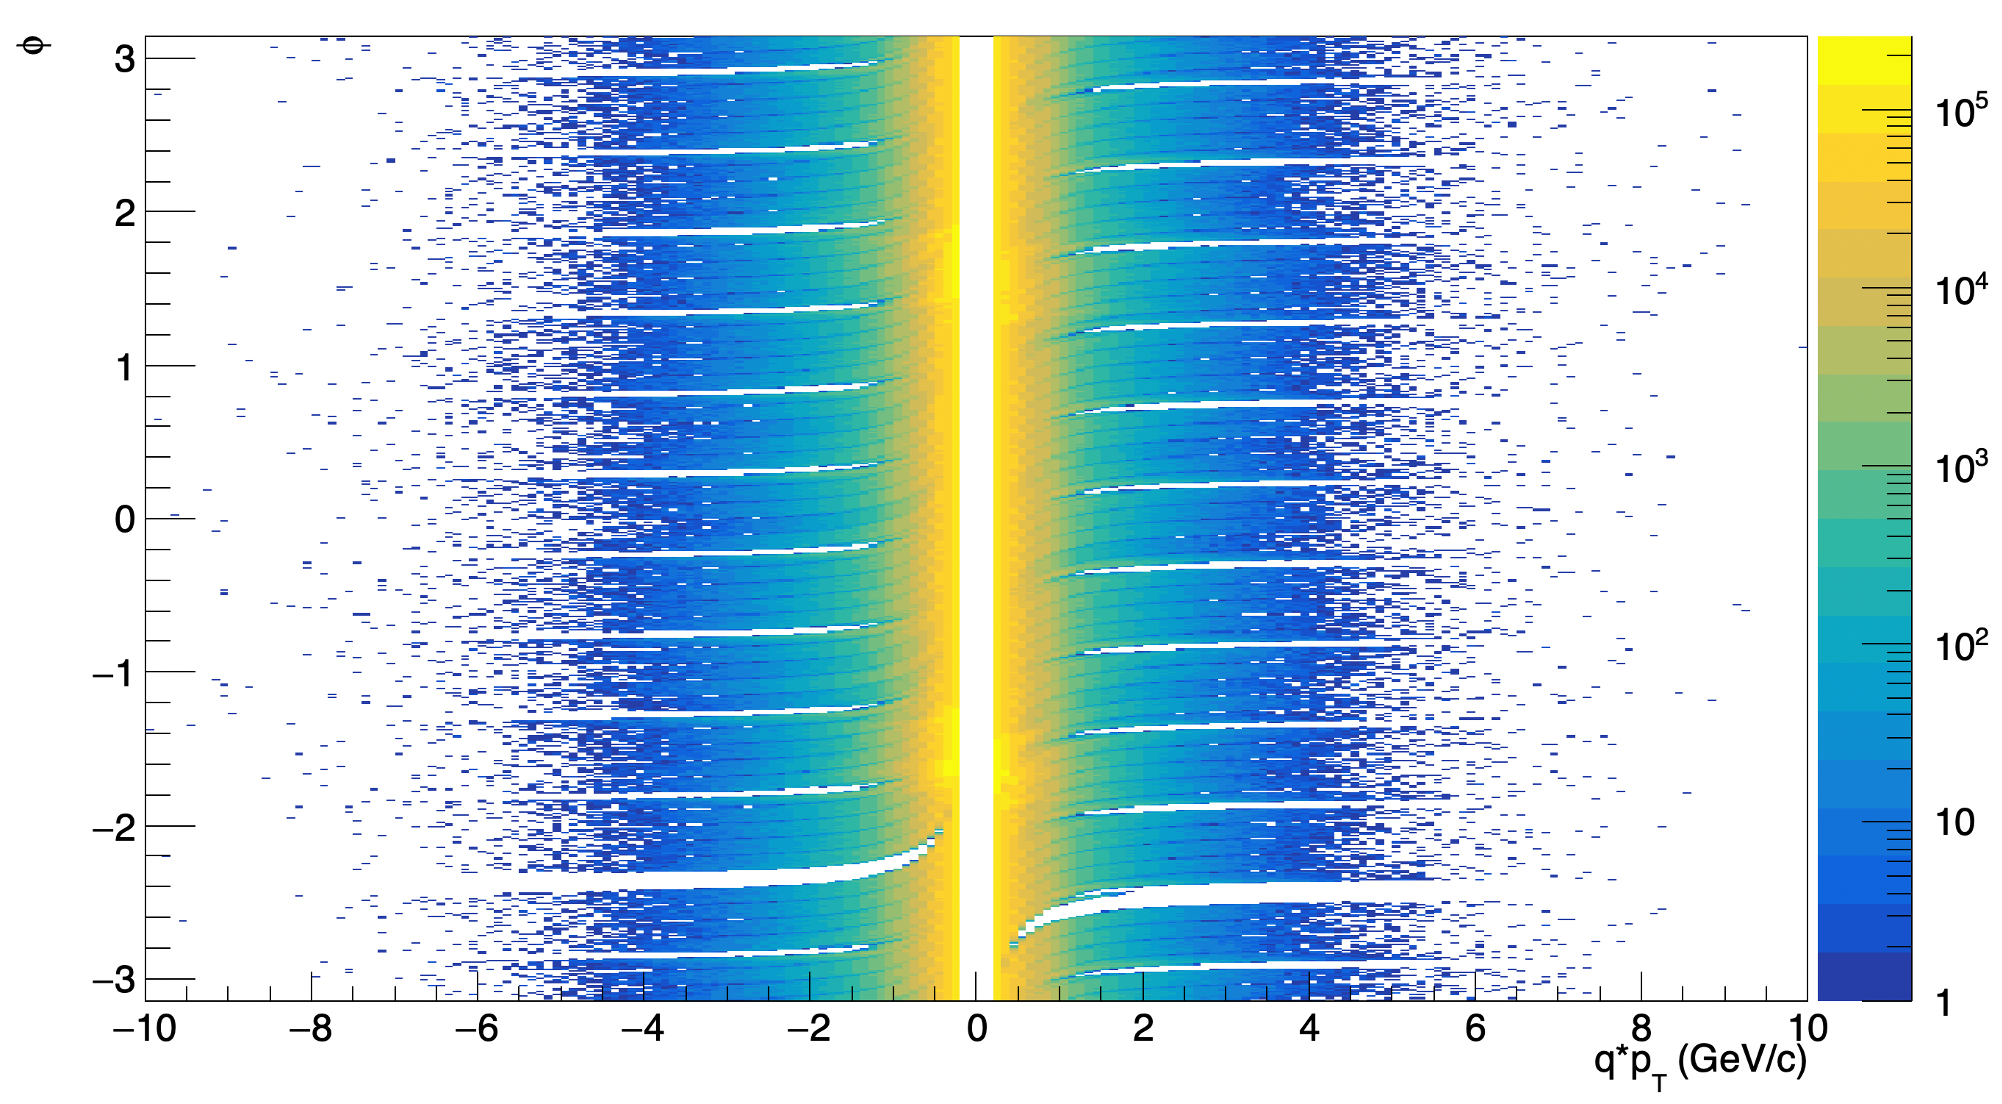
\includegraphics[width=0.75\textwidth,clip]{figures/Chapter4/Phi_vs_Q.png}
  \end{center}
  \caption[电子和正电子在不同横动量下的方位角分布示意图]{电子和正电子在不同横动量下的方位角分布示意图,q>0为正电子,q<0为电子。}
  \label{fig:Phi_vs_Q}
\end{figure}

\subsection{混合事例方法}
\label{chap:mixedEvent}
混合事例方法是将所有的事例按照几个特征来进行分类,再将具有相似特征的不同事例中的电子及正电子进行配对来估计背景。这种方法优点在于统计量高,但缺点是因为是将不同事例中的电子和正电子进行配对,电子和正电子完全不相关,无法重建关联背景。只能在关联背景少的质量区间使用此方法。在本分析中,所有事例通过 \Vz 、中心度(Centrality)和二阶事例平面角(event plane angle, $\Psi_2$)来划分成多个事例库来进行混合。根据 \Vz 和中心度进行分组是为了保证在每一组内都有相似的接收度和探测器探测效率。根据事例平面分组是为了保证在每一组内都有着相似的动量相空间分布,关于二阶事例平面角的计算方式参见\cite{Die:BESI_note}第40页。

确定好分组条件之后,所有事例根据前文当中所提到的划分方式分别被划分到$\rm{20(V_z) \times 9(Centrality) \times 12 (\Psi_2)}$,共2160个事例库当中,每个事例库最多350个事例。当一个事例库达到最大事例数之后,将随机地从库中移除掉一个事例并将最近的事例放入,这将保证所有的事例库中的事例是在不断更新的。就可以避免在事例库被填满之后因为新的事例一直与符合每个库条件的前350个事例进行混合而带来的偏差。

将相同组内的不同事例之间的同号以及异号电子进行配对后可以得到混合事例当中的异号分布(\Bpm)以及同号分布(\Bpp , \Bmm )。通过这三个分布我们可以计算得到电子对接收度的修正因子,如下式所示:
\begin{equation}
  f_{pair~sign~acc.} = \frac{B_{+-}}{2\sqrt{B_{++}B_{--}}}
\end{equation}

\subsection{光子转换背景}
\label{chap:photon_conversion}
在前两个小节当中提到的重建背景的方式主要去除掉的是因为随机配对产生的背景。而在实际的物理分析当中,除了这些因为分析手段引入的背景之外,还有一部分背景是实际存在的物理过程,例如因为光子击中束流管、探测器的支撑结构等位置的时候因为电子对效应所产生的正负电子对。因为这个物理过程并不是我们想要分析的物理过程,所以我们需要通过添加判选条件的方式来对其进行扣除。

为了对这部分背景电子对进行扣除,引入了一个角度$\phi_V$用来进行背景扣除。\PhiV 的定义如式\ref{eq:PhiV}所示。其中$\vec{p_{e+}}$, $\vec{p_{e+}}$ 以及 $\hat{z}$ 分别为正负电子动量和磁场方向矢量。

\begin{equation}
  \begin{split}
      \hat{u} = \frac{ \vec{p_{e+}} + \vec{p_{e-}} }{ |\vec{p_{e+}} + \vec{p_{e-}}| } ~,~ \hat{v} = \frac{ \vec{p_{e+}} \times \vec{p_{e-}} }{ |\vec{p_{e+}} \times \vec{p_{e-}}| }\\
      \hat{w} = \hat{u} \times \hat{v}, \hat{w_z} = \hat{u} \times \hat{z}\\
      cos\phi_V = \frac{\hat{w}~\cdot~\hat{w_z}}{|\hat{w}~\cdot~\hat{w_z}|}
  \end{split}
  \label{eq:PhiV}
\end{equation}

为了更好的理解 \PhiV 角的定义,可以构建以下三个平面:
\begin{itemize}
  \item 平面A:由母粒子的动量方向上的单位向量($\hat{u}$)和z轴的方向上的单位向量($\hat{z}$)构建而成的平面,法向量为$\hat{w_z}$
  \item 平面B:由正负电子电子的动量方向($\vec{p_{e+}}$, $\vec{p_{e+}}$)构建而成的平面,法向量为$\hat{v}$
  \item 平面C:由平面B的法向量方向上的单位向量($\hat{v}$)和母粒子的动量方向上的单位向量($\hat{u}$)构建而成的平面,法向量为$\hat{w}$
\end{itemize}

式\ref{eq:PhiV}中的$\phi_V$即为平面A和C两个平面之间的夹角。又因为平面C垂直于平面B,若定义角$\phi$为A、B两个平面 之间的夹角,则$\phi_V = \phi \pm \frac{\pi}{2}$。对于光子转换过程产生的电子对来说,其$\phi$为$\frac{\pi}{2}$。则光子转换产生的电子对$\phi_V$应为0或者$\pi$。在具体的配对过程当中,会通过固定电子和正电子的顺序的方式来让$\phi_V$趋向于0。而对于随机组合的电子对和来源于强子衰变过程的电子对,这些电子对的$\phi_V$角就没有特殊的倾向。这样就可以通过对$\phi_V$添加判选条件的方式来去掉来自于光子转换的电子对。

图\ref{fig:PhiV_2D}为本分析中转换光子的$\phi_V~\rm{v.s~M_{ee}}$的分布,可以看到转换光子集中在 ${\rm M_{ee} }$< 0.2 GeV 以及 \PhiV 接近于0的区域。在图中可以看到在$\phi_V$接近于0的区域有几个质量不为0的带状分布,
对于光子转换产生的电子对来说,其不变质量应该为0。但是因为本分析中所用的径迹为primary track,在STAR上重建primary track时会要求其通过碰撞顶点。但对于光子转换产生的电子对来说,其产生位置并不在碰撞顶点。这就人为地给光子转换产生的电子对引入了一个张角,导致其电子对质量在最后重建时不为0。不同的光子转换发生位置会引入不同的不变质量。
$\rm{M_{ee}}=\rm{0.01~GeV/c^2}$附近的带状分布为光子击中束流管(beam pile, 距束流管中心约4cm)后产生的转换电子对。$\rm{M_{ee}}=\rm{0.05~GeV/c^2}$附近的带状分布为光子击中内层支架(inner cone supporting structure, 距束流管中心约20cm)后产生的转换电子对。

图\ref{fig:PhiV_2D}中红线为本分析中用到的$\phi_V$角的判选条件条件,这个判选条件和STAR在200 GeV 金-金对撞双电子谱分析中使用的判选条件相同\cite{STAR:2013pwb}。本判选条件的效率通过在计算双电子探测效率时添加相同的判选条件得到。

\begin{figure}[htb]
  \begin{center}
  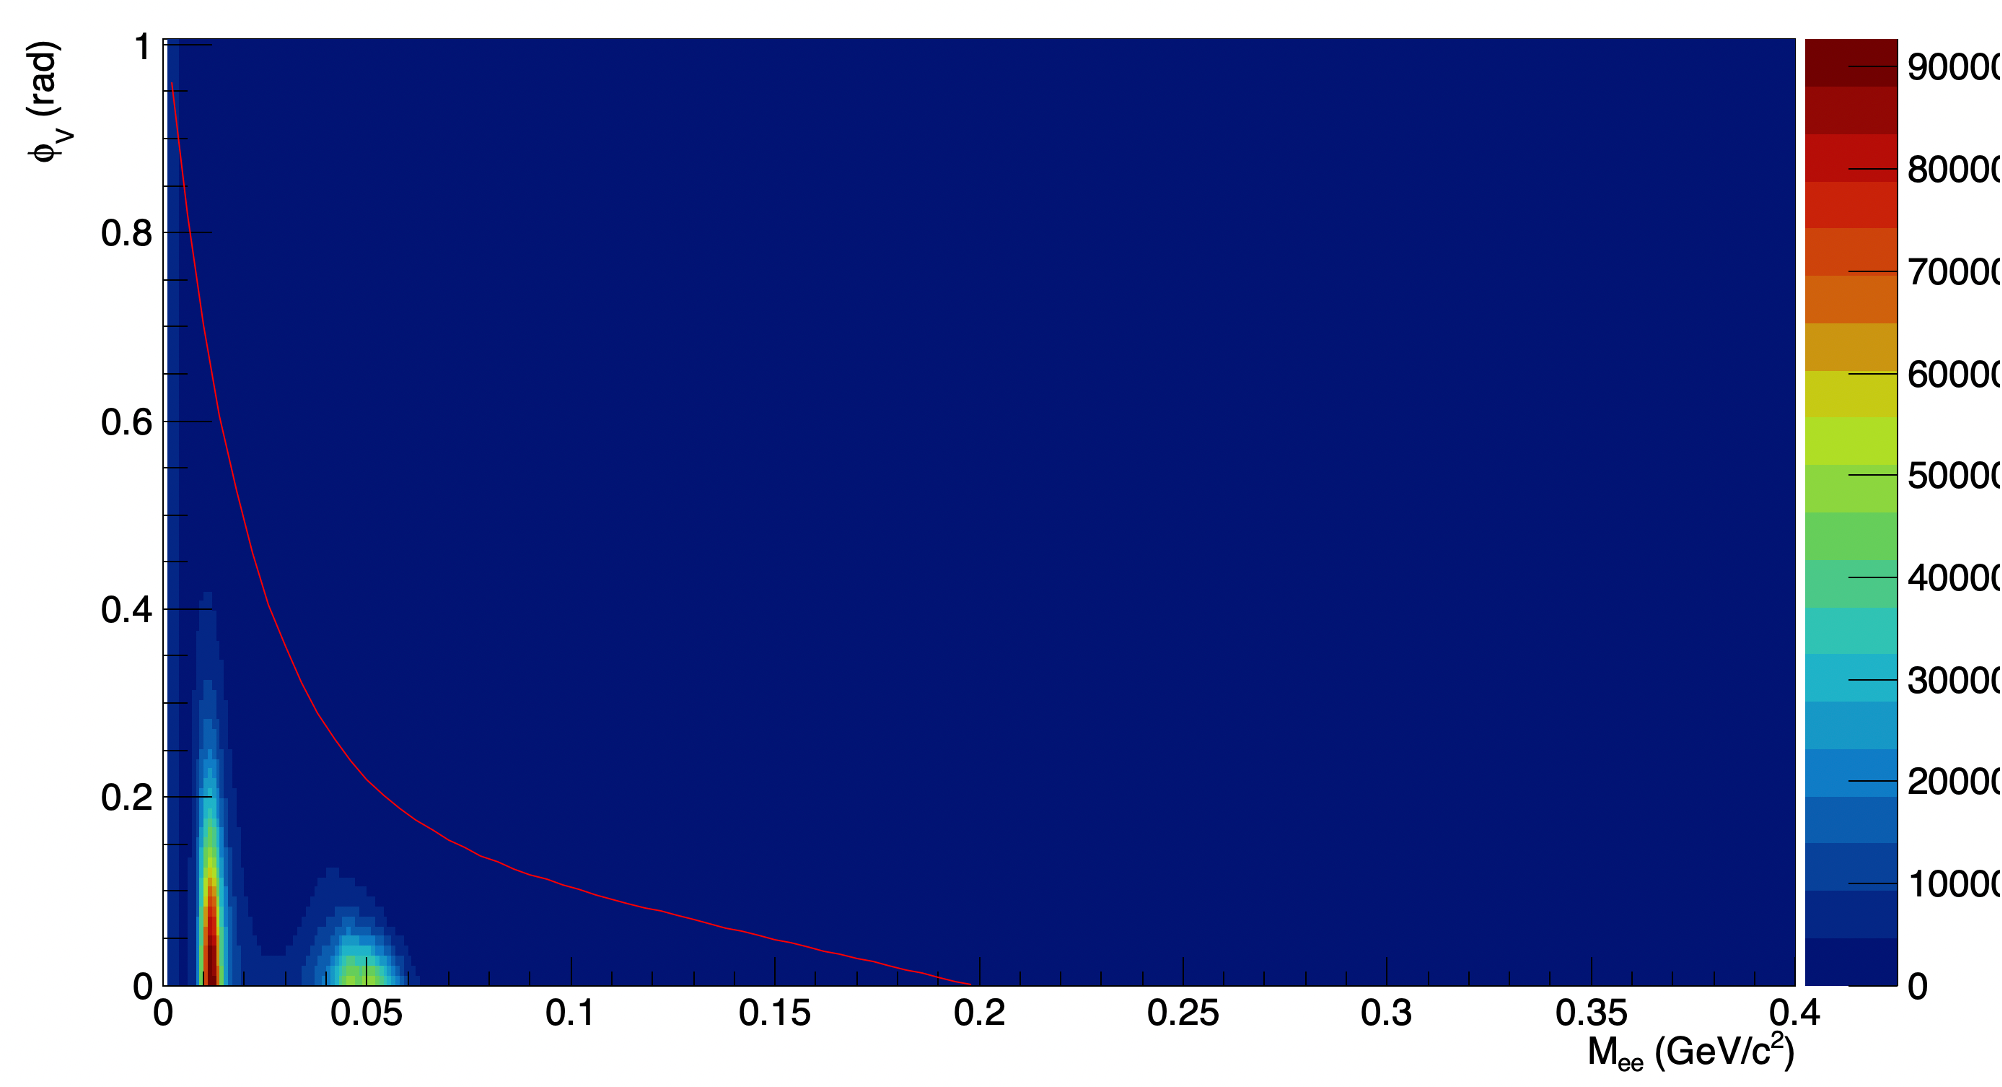
\includegraphics[width=0.75\textwidth,clip]{figures/Chapter4/PhiV_2D.png}
  \end{center}
  \caption[\sNN = 54.4 GeV金-金对撞中的$\phi_v \rm{v.s M_{ee}}$分布示意图]{\sNN = 54.4 GeV金-金对撞中的$\phi_v \rm{~v.s.~M_{ee}}$分布示意图,图上红线为分析所用的$\phi_V$判选条件。}
  \label{fig:PhiV_2D}
\end{figure}

\subsection{原初信号}
\label{chap:raw_signal}
在应用了 \PhiV 判选条件的 \Npm 分布中进行背景扣除即可得到原初信号(raw signal)。计算公式如\ref{eq:raw_signal}所示。这个分布之所以被称为原初信号是因为在此时双电子谱并未经过效率和探测器接收度的修正。这样的双电子谱只能反应在STAR接收度下探测器配置为Run17所用配置的情况下的双电子谱的情况。因为接收度和效率均不相同,无法与其他实验甚至STAR其他能量的结果进行比较。

在STAR实验上测量得到并发表的双电子谱一般有两种,一种是经过了STAR探测器效率修正的双电子谱,即STAR接收度下的双电子谱。另一种是在STAR探测器效率修正的基础上再添加STAR探测器接收度的修正。经过STAR探测器效率修正的双电子谱和介质产生的双电子谱相比相差一个STAR的接收度,可以与STAR其他的效率修正后的测量结果直接比较。但因为不同的探测器的接收度不尽相同,并不能和其他实验的结果直接比较。在经过效率修正的谱上再添加探测器接收度的修正,就可以得到在没有探测器效率以及接收度损失的双电子谱,可以和理论计算以及其他实验经过接收度修正之后的结果进行比较。关于效率修正和探测器接收度修正的部分将在 \ref{chap:efficiency}和\ref{chap:pair_acc}当中讨论。

\begin{equation}
  \label{eq:raw_signal}
  N_{raw~signal} = N_{+-}-N_{bkg}
\end{equation}